\PassOptionsToPackage{table,dvipsnames,svgnames}{xcolor}
\documentclass[
paperwidth=48in,paperheight=36in,
fontscale=0.4
]{baposter}
%\usepackage{babel}
\usepackage{xcolor}             % Define our own colors
\usepackage[font=sf]{caption}  % For Sans serif figure captions
\usepackage{setspace}          % Make things easier to read
\usepackage{enumitem}          % For customising lists
\usepackage{footmisc}          % Customising Footers
\usepackage{titling}           % So we can still use \title and \author
\usepackage{algorithm2e}
\usepackage{algpseudocode}
\usepackage{amsmath,amssymb,amsthm}
\usepackage{graphicx,color}
\usepackage[mathscr]{eucal}
\usepackage{caption,subcaption}
\usepackage{tikz}
\usetikzlibrary{hobby}
\usepackage{pgfplots}
\usepgfplotslibrary{groupplots}

%% Fonts
\usepackage[T1]{fontenc}
\usepackage{tgbonum}
\usepackage[scaled]{helvet}
\usepackage{tgcursor}

%%%%%%%%%%%%%%%%%%%%%%%%%%%%%%%%%%%%%%%%%%%%%%%%%%%%%%%%%%%%%
%% Styling
%%%% Colors
\selectcolormodel{HTML}
\definecolor{rpi-red}{HTML}{e2231b}
%% Footnote Customisation
\renewcommand{\footnotelayout}{\scriptsize\sffamily\raggedright}
%% Line Spacing
\setstretch{1.2}

%% Enum Item
\setitemize{noitemsep,nolistsep}
\setenumerate{noitemsep,nolistsep}
\setdescription{font=\bfseries\sffamily\large\protect\color{black},
   leftmargin=3em}

\title{A New Partitioned Method For Viscous Fluid-Structure Interaction Problems}
\author{ David Wells$^{1,2}$, Jeffrey Banks$^1$, Fengyan Li$^1$               \\
 \vspace{.1in}
 $^1$Rensselaer Polytechnic Institute                                         \\
 \texttt{\small $^2$wellsd2@rpi.edu}                                          \\
 \footnotesize{This work was supported, in part, through the NSF Research Training Groups program (DMS-1344962).}
}

%% Turn off section numbers.
\setcounter{secnumdepth}{-1}
\begin{document}
\begin{poster}{
%%%%%%%%%%%%%%%%%%%%%%%%%%%%%%%%%%%%%%%%%%%%%%%%%%%%%%%%%%%%
% OPTIONS
 grid=no,           % Grid for alignment
 colspacing=1.2em,  % Column spacing
 linewidth=2pt,
 eyecatcher=yes,     % Have no fancy artwork
 columns=3,         % Columns start from 0 i.e. here we have 4
%%%%%%%%%%%%%%%%%%%%%%%%%%%%%%%%%%%%%%%%%%%%%%%%%%%%%%%%%%%%
% Background Options
 background=none,   % do not use a color
 borderColor=rpi-red, %
%%%%%%%%%%%%%%%%%%%%%%%%%%%%%%%%%%%%%%%%%%%%%%%%%%%%%%%%%%%%
 headerColorOne=rpi-red,
 headerColorTwo=rpi-red,
 headershade=plain,
 headerFontColor=white,
 headerborder=open,
 headerheight=0.12\textheight,
 headershape=roundedright,
 headerfont=\Large\sffamily\bfseries,
%%%%%%%%%%%%%%%%%%%%%%%%%%%%%%%%%%%%%%%%%%%%%%%%%%%%%%%%%%%%
 textfont=\sffamily,
 textborder=roundedleft,
 boxColorOne=white,
 boxshade=plain
}
%%%%%%%%%%%%%%%%%%%%%%%%%%%%%%%%%%%%%%%%%%%%%%%%%%%%%%%%%%%%
% Eye Catcher
{ }
% Title
{\sffamily\Huge\thetitle\vspace{-0.2em}}
% Authors
{\sffamily\theauthor}
% University Logo
{
  
\includegraphics[height=0.05\textheight]{RPI_letterhead} \hspace{1.1in}
}

\newcommand*{\vcenterarrow}{\vcenter{\hbox{$\Longrightarrow$}}}
\newcommand*{\vcenterimage}[1]{\vcenter{\hbox{\includegraphics[width=2.5in]{#1}}}}
\newcommand{\leftd}[1]{{\color{red} \bar{#1}}}
\newcommand{\interface}[2]{{\color{blue}{#1}_I(#2)}}
\newcommand{\leftdd}[2]{{\color{red} \bar{#1}(\bar{#2})}}
\newcommand{\leftFourier}[1]{{\color{red} \hat{#1}}}
\newcommand{\leftFourierTwo}[2]{{\color{red} \hat{#1}(\hat{#2})}}
\newcommand{\half}{\dfrac{1}{2}}
\newcommand{\divergence}{\mathrm{div}}

%%%%%%%%%%%%%%%%%%%%%%%%%%%%%%%%%%%%%%%%%%%%%%%%%%%%%%%%%%%%
\headerbox{Partitioned Discretization of a Fluid-Structure Problem}
          {name=Abstract, column=0, row=0}
{
\subsection{Physical Problem}
    \emph{Fluid-Structure Interaction} problems, consisting of a viscous,
    incompressible fluid interacting with an elastic solid, appear in a large
    variety of interesting applications ranging from biological flows [2] to
    free-surface calculations in modeling flows inside the earth's mantle [1].

\subsection{Numerical Discretization}
\begin{itemize}
    \item Discretize both the structure and fluid with continuous finite
          elements
    \item Use of \emph{partitioned} algorithms: fluid and structure equations
          are solved separately at each time step and communicate through a
          well-defined interface
    \item Simplified formulation: resolve individual Fourier modes
    \item Attempt to achieve high-order accuracy (second or better):
          conventional unconditionally stable methods only first-order accurate
\end{itemize}

% \subsection{Results}
%     \begin{itemize}
%         \item Scheme dependent on derivative boundary information
%         \item Numerical results for high-order discretization indicate viability
%               of the scheme
%     \end{itemize}

    \phantom{A}
}


\headerbox{Model Problem}
          {name=Intro, column=0, below=Abstract, above=bottom}
{
\begin{center}
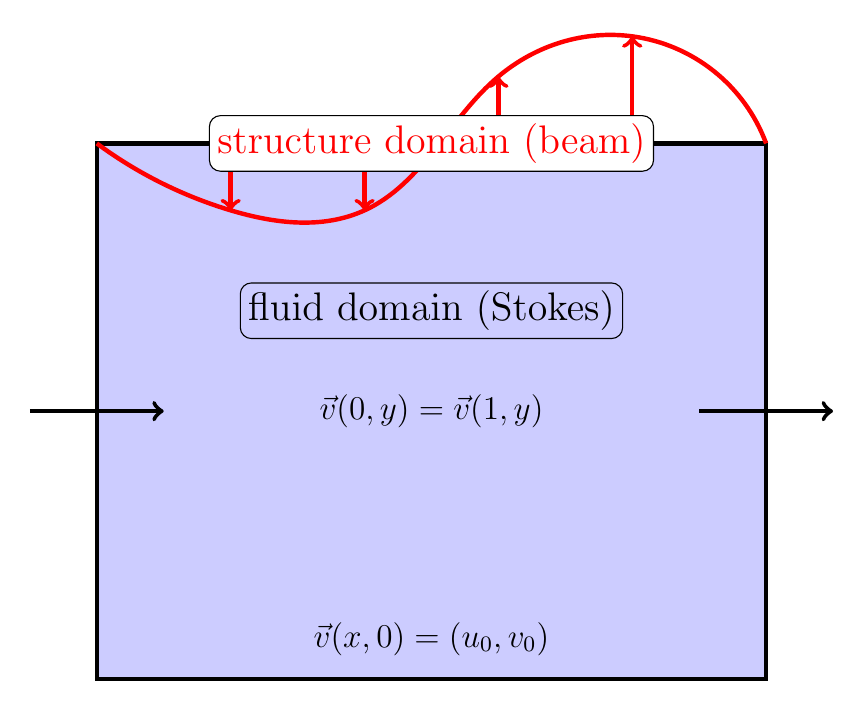
\begin{tikzpicture}[scale=1.7]
  % \useasboundingbox (0,.5) rectangle (16,5);  % set the bounding box (so we have less surrounding white space)
  \draw[fill=blue!20,draw=black,ultra thick] (0,0) rectangle (5cm,4cm);

  %% beam stuff
  % \draw[red] (0,5) .. controls (1.25,4.4) and (3.75, 5.8) .. (5,5);
  \draw[red, ultra thick] (0, 4) to [curve through = {(1., 3.5) .. (2.0, 3.5) .. (3.0, 4.5) .. (4.0, 4.8)}] (5,4);
  % \draw (0, 0) to [curve through = {(6, 4) .. (4, 9 ) .. (1, 7)}] (3, 5);
  \draw[->,ultra thick, red] (1.0, 4.0) -- (1.0, 3.5);
  \draw[->,ultra thick, red] (2.0, 4.0) -- (2.0, 3.5);
  \draw[->,ultra thick, red] (3.0, 4.0) -- (3.0, 4.5);
  \draw[->,ultra thick, red] (4.0, 4.0) -- (4.0, 4.8);

  %% fluid periodicity
  \draw[->, ultra thick] (-0.5,2) -- (0.5,2);
  \draw[->, ultra thick] (4.5,2) -- (5.5,2);
  \draw(2.5, 2) node[rounded corners] {\color{black}\large \(\vec{v}(0, y) = \vec{v}(1, y)\)};

  %% fluid bottom BC
  \draw(2.5, 0.3) node[rounded corners] {\color{black}\large \(\vec{v}(x, 0) = (u_0, v_0)\)};

  %% labels
  \draw(2.5,2.75) node[draw,fill=blue!20,rounded corners, inner sep=0.1cm] {\color{black}\Large fluid domain (Stokes)};
  \draw(2.5, 4.0) node[draw,fill=white,rounded corners,inner sep=.1cm]{\color{red}\Large structure domain (beam)};
\end{tikzpicture}
\end{center}
% }
% %%%%%%%%%%%%%%%%%%%%%%%%%%%%%%%%%%%%%%%%%%%%%%%%%%%%%%%%%%%%

% \headerbox{Governing Equations}
%           {name=Formulation, column=0, below=Intro, above=bottom}
% {
\begin{itemize}
    \item Model the structure with a beam equation (position \(\leftd{u}\),
          velocity \(\leftd{v}\), fluid traction force \(\leftd{b}\), external
          force \(\leftd{f}\)):
          \begin{align*}
              \leftd{u}_{\color{red}t}              &= \leftd{v}              \\
              \leftd{\rho} \leftd{v}_{\color{red}t} &= \leftdd{\mathcal{L}}{u} +
              \leftd{b} + \leftd{f}                                           \\
              \leftdd{\mathcal{L}}{u}  &= \leftd{s} \leftd{u}_{\color{red}xx}
              - \leftd{a} \leftd{u}_{\color{red}xxxx}
          \end{align*}

    \item Model the incompressible, viscous fluid with the Stokes equations
          (velocity \(\vec{v}\), pressure \(p\), viscosity \(\nu\), density
          \(\rho\), external force \(\vec{f}\)):
          \begin{align*}
              \rho \vec{v}_t &= \divergence(\sigma) + \vec{f}                 \\
              \sigma &= -p I + 2 \nu \varepsilon(v)                           \\
              \varepsilon(\vec{v})_{ij} &= \dfrac{1}{2}
              \left(
              \dfrac{\partial v_i}{\partial x_j} +
              \dfrac{\partial v_j}{\partial x_i}
              \right)                                                         \\
              \divergence(\vec{v}) &= 0
          \end{align*}

    \item These are coupled \emph{at a continuous, but not necessarily discrete,
          level} with no-slip boundary conditions and the body force definition:
          \begin{align*}
              \vec{v}   &= \leftd{v} \text{ (at the interface)}               \\
              \leftd{b} &= -\sigma \vec{n}
          \end{align*}
\end{itemize}
}
%%%%%%%%%%%%%%%%%%%%%%%%%%%%%%%%%%%%%%%%%%%%%%%%%%%%%%%%%%%%%
%%%%%%%%%%%%%%%%%%%%%%%%%%%%%%%%%%%%%%%%%%%%%%%%%%%%%%%%%%%%
\headerbox{The Added-Mass Instability}
          {name=AddedMass,column=1}
{
\begin{center}
    \includegraphics[width=2.5in]{left.png}
    \hspace{0.5in}
    \includegraphics[width=2.5in]{right.png}
\end{center}

\vspace{-0.5in}

Consider a low density solid either immersed in a fluid or in a vacuum. If we
apply a force to the body in the vacuum then its acceleration will be
proportional to the force. If we apply a force to the body in a fluid then the
drag force will dominate: this effect is neglected in the traditional algorithm.
We can resolve this instability [2] by using the traction condition for the
structure and matching \emph{accelerations} for the fluid instead:

\begin{align*}
    \leftd{\rho} \leftd{h} \leftd{v}_{{\color{red}t}}
    &= \leftdd{\mathcal{L}}{u} + \leftd{f} - \sigma \vec{n}
    \quad \text{ (beam equation)}                                             \\
    \leftd{\rho} \leftd{h} v_t
    &= \leftdd{\mathcal{L}}{u} + \leftd{f} - \sigma \vec{n}
    \quad \text{ (equal acceleration)}                                        \\
    \dfrac{\leftd{\rho} \leftd{h}}{\rho} \divergence(\sigma)
    + \dfrac{\leftd{\rho} \leftd{h}}{\rho} f
    &= \leftdd{\mathcal{L}}{u} + \leftd{f} - \sigma \vec{n}
    \quad \text{ (Stokes equations)}
\end{align*}

\begin{equation*}
    \sigma \vec{n} + \dfrac{\leftd{\rho} \leftd{h}}{\rho} \divergence(\sigma)
    = \leftdd{\mathcal{L}}{u}
    + \leftd{f}
    - \dfrac{\leftd{\rho} \leftd{h}}{\rho} \vec{f}.
\end{equation*}

\phantom{A}
}

%%%%%%%%%%%%%%%%%%%%%%%%%%%%%%%%%%%%%%%%%%%%%%%%%%%%%%%%%%%%
\headerbox{Weak Form and Finite Element Discretization}
{name=FEScheme,column=1,below=AddedMass,above=bottom}
{
\begin{itemize}
    \item Apply the Fourier transform:
          \begin{align*}
              \begin{pmatrix}
                  \hat{u} \\ \hat{v}
              \end{pmatrix}_t
              &=
              \begin{pmatrix}
                  i k & \dfrac{\partial}{\partial y}
              \end{pmatrix}
              \cdot
              \left[
              \begin{pmatrix}
                  -\hat{p} \vphantom{\dfrac{1}{2}} & 0                        \\
                  0 \vphantom{\dfrac{1}{2}}        & -\hat{p}
              \end{pmatrix}
              +
              2 \nu
              \begin{pmatrix}
                  i k \hat{u} & \dfrac{1}{2} \left(\hat{u}_y + i k \hat{v}\right)\\
                  \dfrac{1}{2} \left(\hat{u}_y + i k \hat{v}\right) & \hat{v}_y
              \end{pmatrix}
              \right]
              +
              \begin{pmatrix}
                  \hat{f}_0 \vphantom{\dfrac{1}{2}}                           \\
                  \hat{f}_1 \vphantom{\dfrac{1}{2}}
              \end{pmatrix}                                                   \\
              0 &=
              \left(i k, \dfrac{\partial}{\partial y}\right) \cdot (\hat{u},
              \hat{v})
          \end{align*}

    \item Weak form:
          \begin{align*}
              (\varphi_0, \hat{u})_t
              &=
              -2 \nu k^2 (\varphi_0, \hat{u})
              - \nu (\varphi_{0,y}, \hat{u}_y + i k \hat{v})
              - i k (\varphi_0, \hat{p})
              + (\varphi_0, \hat{f}_0)                                        \\
              (\varphi_1, \hat{v})_t
              &=
              -2 \nu (\varphi_{1,y}, \hat{v}_y)
              + \nu (\varphi_1, i k \hat{u}_y - k^2 \hat{v})
              + (\varphi_{1,y}, \hat{p})                                      \\
              &\phantom{=} + (\varphi_1, \hat{f}_1)
              + \varphi_1(1) (2 \nu \hat{v}_y(1) - \hat{p}(1))
              \nonumber                                                       \\
              (q, i k \hat{u} + \hat{v}_y)
              &= 0
          \end{align*}

    \item AMP boundary condition for the fluid:
          \begin{equation*}
              2 \nu \hat{v}_y(1) - \hat{p}(1)
              =
              \leftdd{\mathcal{L}}{u}{\color{red}(1)}
              +
              \leftd{f}{\color{red}(1)}
              +
              \dfrac{\leftd{\rho}\leftd{h}}{\rho}
              \hat{f}_1(1)
              -
              \dfrac{\leftd{\rho}\leftd{h}}{\rho}
              \left(\nu (-k^2 \hat{v}(1) - i k \hat{u}_y(1)) + \hat{p}_y(1)\right)
          \end{equation*}

    \item Enforce derivative conditions in pressure and velocity with derivative
          basis functions:
\end{itemize}
\begin{center}
    % \begin{tikzpicture}[scale=0.25]
    %     \begin{axis}[xmin=0,
    %         % hide axis,
    %         xmax=1,
    %         no markers,
    %         xtick={0, 1},
    %         ytick={0, 1}]
    %         \addplot[samples=100,color=red] {(1 - x)^2};
    %         \addplot[samples=100,color=blue] {x*(x - 1)};
    %         \addplot[samples=100,color=teal] {x*(2 - x)};
    %     \end{axis}



    %     \begin{axis}[xmin=0,
    %         % hide axis,
    %         xmax=1,
    %         no markers,
    %         xtick={0, 1},
    %         ytick={0, 1}]
    %         \addplot[samples=100,color=red] {(1 - x)^2};
    %         \addplot[samples=100,color=blue] {x*(x - 1)};
    %         \addplot[samples=100,color=teal] {x*(2 - x)};
    %     \end{axis}
    % \end{tikzpicture}
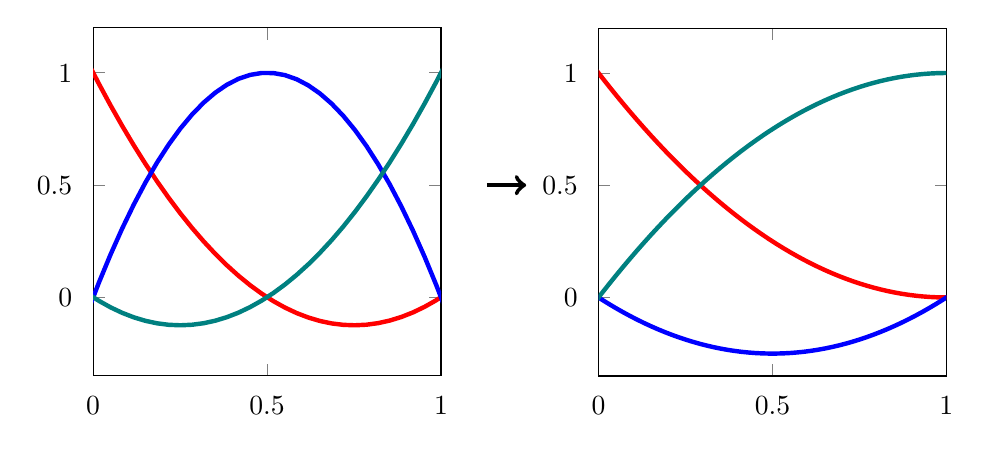
\begin{tikzpicture}
    \begin{axis}[name=plot1,
        width=6cm,
        height=6cm,
        xmin=0,
        % hide axis,
        xmax=1,
        ymin=-0.35,
        ymax=1.2,
        xtick={0, 0.5, 1},
        ytick={0, 0.5, 1},
        xticklabel style={yshift=-4pt},
        yticklabel style={xshift=-4pt},
        ]
        \addplot[samples=300,color=red, ultra thick] {2*(x - 0.5)*(x - 1)};
        \addplot[samples=300,color=blue, ultra thick] {-4*(x - 0)*(x - 1)};
        \addplot[samples=300,color=teal, ultra thick] {2*(x - 0)*(x - 0.5)};
    \end{axis}
    \draw[->, ultra thick] (5,2.425) -- (5.5,2.425);

    \begin{axis}[name=plot2,
        at={($(plot1.east) + (2cm,0)$)},
        anchor=west,
        width=6cm,
        height=6cm,
        xmin=0,
        xmax=1,
        ymin=-0.35,
        ymax=1.2,
        xtick={0, 0.5, 1},
        ytick={0, 0.5, 1},
        xticklabel style={yshift=-4pt},
        yticklabel style={xshift=-4pt},
        ]
        \addplot[samples=500,color=red, ultra thick] {(1 - x)^2};
        \addplot[samples=500,color=blue, ultra thick] {x*(x - 1)};
        \addplot[samples=500,color=teal, ultra thick] {x*(2 - x)};
    \end{axis}
\end{tikzpicture}


    % \begin{equation*}
    %     \vcenterimage{lagrange-quadratics.png}
    %     \vcenterarrow
    %     \vcenterimage{hermite-quadratics.png}
    % \end{equation*}
\end{center}
\phantom{A}
}

\headerbox{Numerical Results} {name=NumericalResults,column=2,row=0}
{
\subsection{Experimental Setup}
    \begin{itemize}
        \item Method of manufactured solutions with a stream function:
              \begin{align*}
                  \psi(t, y) &= t \sin(3.3 t y) \cos(3 y) \exp(4 y)           \\
                  p(t, y)    &= t y (5 - y)^2 \exp(-3 y) \sin(5 t)
              \end{align*}
        \item Finite elements: Taylor-Hood (\(P^3-P^2\) pair) in 1D
        \item Time integrator: trapezoid rule, \(\Delta t = \Delta y^2\),
              extrapolated traction for the structure solver
    \end{itemize}
\subsection{Convergence Rates for \(\leftd{\rho}/\rho = 100\)}
    This case represents a beam with density \(100\) times greater than that
    of the fluid: the added-mass effect does not play a significant role
    here.
    \begin{center}
        \begin{tabular}{| l | l | l | l | l | l | l | l |}
            \hline
            \(k\) & \texttt{n\_cells} &
            \(\hat{p}\) error & \(\hat{v}\) error & \(\leftFourier{v}\) error &
            \(\hat{p}\) rate & \(\hat{v}\) rate & \(\leftFourier{v}\) rate    \\
            \hline
            0 & 20 & 1.06e-01 & 3.13e-04 & 1.05e-04 & 1.44 & 3.98 & 1.44      \\
            0 & 40 & 2.96e-02 & 1.96e-05 & 2.93e-05 & 1.89 & 3.99 & 1.89      \\
            0 & 60 & 1.35e-02 & 3.88e-06 & 1.34e-05 & 1.93 & 3.99 & 1.93      \\
            0 & 80 & 7.71e-03 & 1.22e-06 & 7.65e-06 & 1.95 & 3.99 & 1.95      \\
            \hline
            1 & 20 & 2.52e+00 & 1.26e-01 & 2.01e-03 & 2.73 & 2.65 & 2.59      \\
            1 & 40 & 3.42e-01 & 1.77e-02 & 2.92e-04 & 2.90 & 2.87 & 2.82      \\
            1 & 60 & 1.04e-01 & 5.44e-03 & 9.09e-05 & 2.94 & 2.92 & 2.89      \\
            1 & 80 & 4.44e-02 & 2.33e-03 & 3.93e-05 & 2.95 & 2.94 & 2.92      \\
            \hline
        \end{tabular}
    \end{center}

\subsection{Convergence Rates for \(\leftd{\rho}/\rho = 0.01\)}
    This case represents a beam with density \(100\) times \emph{smaller} than that
    of the fluid: in this case the added-mass effect dominates and the
    traditional algorithm will be unstable.
    \begin{center}
        \begin{tabular}{| l | l | l | l | l | l | l | l |}
            \hline
            \(k\) & \texttt{n\_cells} &
            \(\hat{p}\) error & \(\hat{v}\) error & \(\leftFourier{v}\) error &
            \(\hat{p}\) rate & \(\hat{v}\) rate & \(\leftFourier{v}\) rate    \\
            \hline
            0 & 20 & 1.74e-04 & 4.26e-07 & 4.07e-05 & 2.86 & 3.72 & 5.18      \\
            0 & 40 & 2.31e-05 & 2.95e-08 & 1.73e-05 & 2.92 & 3.88 & 0.00      \\
            0 & 60 & 7.06e-06 & 6.03e-09 & 1.05e-05 & 2.92 & 3.92 & 1.42      \\
            0 & 80 & 3.05e-06 & 1.94e-09 & 6.57e-06 & 2.91 & 3.94 & 1.69      \\
            \hline
            1 & 20 & 1.35e+00 & 4.86e-02 & 1.28e+00 & 3.16 & 3.05 & 3.81      \\
            1 & 40 & 1.56e-01 & 5.86e-03 & 9.47e-02 & 3.09 & 3.04 & 3.73      \\
            1 & 60 & 4.51e-02 & 1.71e-03 & 2.14e-02 & 3.06 & 3.03 & 3.64      \\
            1 & 80 & 1.87e-02 & 7.18e-04 & 7.61e-03 & 3.05 & 3.02 & 3.57      \\
            \hline
        \end{tabular}
    \end{center}

\phantom{A}
}

%%%%%%%%%%%%%%%%%%%%%%%%%%%%%%%%%%%%%%%%%%%%%%%%%%%%%%%%%%%%k
\headerbox{Conclusions}
          {name=SummaryAndFuture,column=2,below=NumericalResults}
{
\subsection{Summary}
    Partitioned methods allow for one to use standard algorithms, with some
    changes to boundary condition implementations, to solve fluid-structure
    interaction problems. This work shows that it is possible to resolve some
    stability problems with fluid-structure interaction problems through the use
    of special boundary conditions.

\subsection{Future Work}
    \begin{itemize}
        \item Fix order of accuracy loss in fluid velocity (likely due to
              boundary derivatives)
        \item Establish energy estimates proving stability for the discrete
              system
        \item Extend to structures with nonzero \(x\) displacement
    \end{itemize}
}
%%%%%%%%%%%%%%%%%%%%%%%%%%%%%%%%%%%%%%%%%%%%%%%%%%%%%%%%%%%%k

\headerbox{Citations}
          {name=Citations,column=2,below=SummaryAndFuture,above=bottom}
{
\begin{enumerate}
    \item W. Bangerth, J. Dannberg, R. Gassm{\"o}ller, T. Heister et al.
          \textsc{ASPECT}: Advanced Solver for Problems in Earth's ConvecTion,
          User Manual. \texttt{DOI:10.6084/m9.figshare.4865333}
    \item L. Li, W. Henshaw, J. Banks, D. Schwendeman, and G. Main. \emph{A
          stable partitioned FSI algorithm for incompressible flow and deforming
          beams}. \texttt{arXiv:1507.06041}, 2016
\end{enumerate}
}
%%%%%%%%%%%%%%%%%%%%%%%%%%%%%%%%%%%%%%%%%%%%%%%%%%%%%%%%%%%%

%%%%%%%%%%%%%%%%%%%%%%%%%%%%%%%%%%%%%%%%%%%%%%%%%%%%%%%%%%%%


\end{poster}%
\end{document}
